\documentclass{article}
\usepackage{amsmath}
\usepackage{amsfonts}
\usepackage{amssymb}
\usepackage{amsmath}
\usepackage{amsthm}
\usepackage{bm}
\usepackage{changepage}
\usepackage{esint}
\usepackage{framed}
\usepackage{geometry}
\usepackage{inputenc}
\usepackage{mathrsfs}
\usepackage{mathtools}
\usepackage{marvosym}
\usepackage{tikz}
\usepackage{times}
\usepackage{xcolor}

\title{Math 4500 HW \#12 Solutions}
\author{Instructor: Birgit Speh\\ TA: Guanyu Li}
\date{}
\geometry{left=2cm,right=2cm,top=2.5cm,bottom=2.5cm}

\theoremstyle{definition}
\newtheorem{problem}{Problem}
\theoremstyle{plain}
\newtheorem*{remark}{Remark}

\begin{document}

\maketitle\par

\emph{This solution set is not error-free. Please email me (gl479\MVAt cornell.edu) if you spot any errors or typos!}

\begin{problem}[Exercise 7.6.3 (10 pts)]
Suppose that $e^Xe^Y=e^Ye^X$. Show that $XY=YX$.
\end{problem}
\begin{adjustwidth}{0.7cm}{}
\color{blue}
\begin{proof}[Solution]
Suppose that $X=\log(I+(e^X-I))$ and $Y=\log(I+(e^Y-I))$, then we know that
\begin{align*}
\\
&=\sum_{n=1}^{+\infty}(-1)^{n-1}(e^X-I)^n\sum_{n=1}^{+\infty}(-1)^{n-1}(e^Y-I)^n\\
&=\sum_{n,m=1}^{+\infty}(-1)^{n+m}(e^X-I)^n(e^Y-I)^m.
\end{align*}
Since that $e^Xe^Y=e^Ye^X$, we have $(e^X-I)^n(e^Y-I)^m=(e^Y-I)^m(e^X-I)^n$, thus
\begin{align*}
\sum_{n,m=1}^{+\infty}(-1)^{n+m}(e^X-I)^n(e^Y-I)^m&=\sum_{n,m=1}^{+\infty}(-1)^{n+m}(e^Y-I)^m(e^X-I)^n\\
&=\log(I+(e^Y-I))\log(I+(e^X-I))=YX.
\end{align*}
\color{black}
\end{proof}
\end{adjustwidth}

\begin{problem}[Exercise 7.6.4 (8 pts)]
Deduce from Exercise 7.6.3. that $e^Xe^Y=e^{X+Y}$ if and only if $XY=YX$.
\end{problem}
\begin{adjustwidth}{0.7cm}{}
\color{blue}
\begin{proof}[Solution]
Since $X+Y=Y+X$, if $e^Xe^Y=e^{X+Y}$ then
\begin{displaymath}
e^Xe^Y=e^{X+Y}=e^{Y+X}=e^Ye^X,
\end{displaymath}
and by previous problem, $XY=YX$. Converse proposition was proved in the text.
\color{black}
\end{proof}
\end{adjustwidth}

\begin{problem}[Exercise 9.1.1 (7 pts)]
Find algebraic properties showing that the groups $O(2),SO(2)$, and $\mathbb{R}$ are not isomorphic.
\end{problem}
\begin{adjustwidth}{0.7cm}{}
\color{blue}
\begin{proof}[Solution]
Notice that $O(2)$ is not abelian and the other two are abelian. There are elements in $SO(2)$ with finite orders, i.e. $\mathbb{Z}/n\mathbb{Z}$ is a subgroup of $SO(2)$, but for any $0\neq r\in\mathbb{R}$, if $nr=0$ for some integer $n$, then $n=0$.
\color{black}
\end{proof}
\end{adjustwidth}

\begin{problem}[Exercise 9.1.2 (5 pts)]
Explain why it is appropriate to call $S^1\times S^1$, $S^1\times\mathbb{R}$ and $\mathbb{R}\times\mathbb{R}$ the torus, cylinder, and plane respectively.
\end{problem}
\begin{adjustwidth}{0.7cm}{}
\color{blue}
\begin{proof}[Solution]
$S^1\times S^1$ is gluing opposite sides of a square, say
\begin{center}
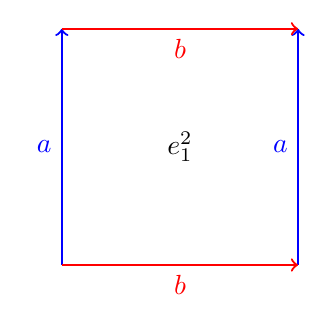
\begin{tikzpicture}
\draw [thick,blue,->] (0,0) -- (0,3) node [left] at (0,1.5) {$a$};
\draw [thick,blue,->] (3,0) -- (3,3) node [left] at (3,1.5) {$a$};
\draw [thick,red,->] (0,0) -- (3,0) node [below] at (1.5,0) {$b$};
\draw [thick,red,->] (0,3) -- (3,3) node [below] at (1.5,3) {$b$};
\node at (1.5,1.5) {$e_1^2$};
\end{tikzpicture}.
\end{center}
If we find a representative of it in $\mathbb{R}^3$, the gluing process gives us a torus. Similar to $S^1\times\mathbb{R}$, this is the gluing of a infinitely long stripe, which gives us a(n) (infinitely long) cylinder.
\color{black}
\end{proof}
\end{adjustwidth}

\begin{problem}[Exercise 9.1.3 (10 pts)]
Show that the three groups have the same Lie algebra. Describe its underlying vector space and Lie bracket operation.
\end{problem}
\begin{adjustwidth}{0.7cm}{}
\color{blue}
\begin{proof}[Solution]
By definition, the Lie algebra of a group is the set of the tangent vectors of all possible smooth paths going through the identity. But the tangent vector is a local notion, it suffices to prove that these three groups have the same local property at the identity. Notice that $S^1\times S^1\cong\mathbb{R}^2/\mathbb{Z}^2$ and $S^1\times\mathbb{R}\cong\mathbb{R}^2/\mathbb{Z}$, so there are open neighborhoods of the identities of the three groups s.t. they are homeomorphic, hence they have the same Lie algebra.\par
If we just compute the Lie algebra of $\mathbb{R}\times\mathbb{R}$, the underlying space is $\mathbb{R}\times\mathbb{R}$, with the trivial bracket.
\color{black}
\end{proof}
\end{adjustwidth}

\begin{problem}[Exercise 9.1.4 (15 pts)]
Distinguish the three groups algebraically and topologically.
\end{problem}
\begin{adjustwidth}{0.7cm}{}
\color{blue}
\begin{proof}[Solution]
Algebraically, $\mathbb{Z}/n\mathbb{Z}\times\mathbb{Z}/n\mathbb{Z}$ is a subgroup of $S^1\times S^1$, but not a subgroup of $S^1\times\mathbb{R}$ nor $\mathbb{R}\times\mathbb{R}$. We only need to prove that $\mathbb{Z}/n\mathbb{Z}\times\mathbb{Z}/n\mathbb{Z}$ is not a subgroup of $S^1\times\mathbb{R}$. Suppose not, then we have some injection $\varphi:\mathbb{Z}/n\mathbb{Z}\times\mathbb{Z}/n\mathbb{Z}\to S^1\times\mathbb{R}$, then since all elements in $\mathbb{Z}/n\mathbb{Z}\times\mathbb{Z}/n\mathbb{Z}$ are of finite order, so their image under $\varphi$. Thus $\mathrm{Im}~\varphi\subseteq S^1\times\{0\}$. But $\mathbb{Z}/n\mathbb{Z}\times\mathbb{Z}/n\mathbb{Z}$ is not cyclic but all finite subgroup of $S^1$ is cyclic, a contradiction. Similarly, $\mathbb{Z}/n\mathbb{Z}$ is a subgroup of $S^1\times\mathbb{R}$ but not of $\mathbb{R}\times\mathbb{R}$.\par
Topologically, $S^1\times S^1$ is compact but not simply connected, while $S^1\times\mathbb{R}$ is noncompact but not simply connected. $\mathbb{R}\times\mathbb{R}$ is noncompact but simply connected.
\color{black}
\end{proof}
\end{adjustwidth}

\end{document} 